\section{Pro/Kontra} % (fold)
\label{sec:pro_kontra}
\subsection*{subsection name} % (fold)
\label{sub:subsection_name}

% subsection subsection_name (end)
\begin{frame}
	\frametitle{Pro/Kontra}
	\begin{block}{Pro Kryo-TEM}
		\begin{itemize}
			\item Hohe Auflösung bei Größen von $\SIrange[range-phrase = -]{0.5}{100}{\mega\dalton}$			
			\item Native Konformation wird beibehalten
			\item Schnelles lösen von groben Strukturen
		\end{itemize}
	\end{block}
	\begin{block}{Kontra Kryo-TEM}
		\begin{itemize}
			\item Probleme bei Größen von $\SIrange[range-phrase = -]{0.1}{0.5}{\mega\dalton}$
			\item Maximale Auflöung $\SIrange[range-phrase = -]{2}{3}{\angstrom}$
			\item Sehr viele Partikel vonnöten
		\end{itemize}
	\end{block}
	\begin{figure}
		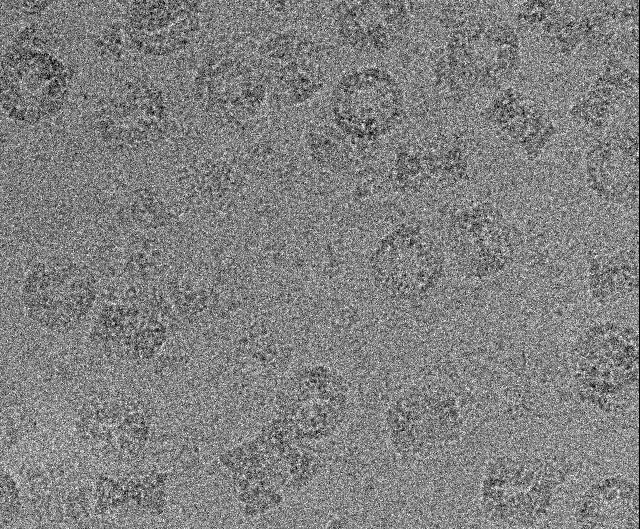
\includegraphics[height = 2.5cm]{pic/kryo1.png}
	\end{figure}
\end{frame}

\begin{frame}
	\frametitle{Pro/Kontra}
	\begin{block}{Pro Kristallographie}
		\begin{itemize}
			\item Atomare Auflösung
			\item "`Einfaches"' Lösen der Primärstruktur
		\end{itemize}
	\end{block}
	\begin{block}{Kontra Kristallographie}
		\begin{itemize}
			\item Nicht alle Proben sind leicht zu kristallisieren
			\item Keine Aussage über die native Konformation
			\item Zerstörung der Struktur
		\end{itemize}
	\end{block}
	\begin{figure}
		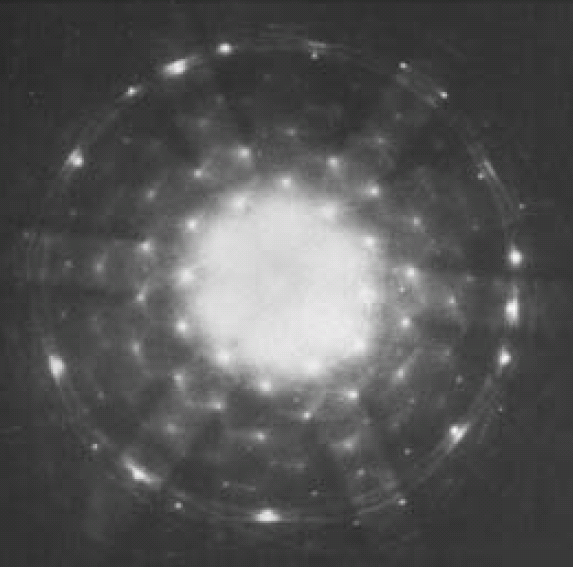
\includegraphics[height = 3cm]{pic/kristall.png}
	\end{figure}
\end{frame}

\begin{frame}
	\frametitle{Pro/Kontra}
	\begin{block}{Pro Tomographie}
		\begin{itemize}
			\item Bekannte Projektionsparameter
			\item Geeignet für Zellen oder Organellen
		\end{itemize}
	\end{block}
	\begin{block}{Kontra Tomographie}
		\begin{itemize}
			\item Zerstört leicht biologische Proben
			\item Nicht alle Raumwinkel abdeckbar
		\end{itemize}
	\end{block}
	\begin{figure}
		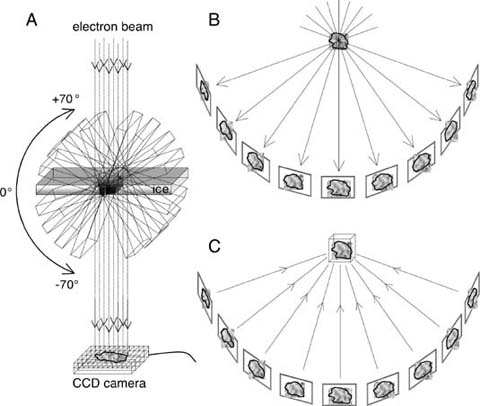
\includegraphics[height = 3.5cm]{pic/tomography.jpg}
	\end{figure}
\end{frame}